\section{TECHNICAL FOUNDATIONS OF O-ISAC}
\label{sec:foundations_comparison}

The physical interaction that enables sensing also determines how it can
share resources with communication. This section follows the signal from
that interaction to the receiver, then explains the optical constraints on
sharing and the measures used to evaluate both functions.
Numerical examples show how a shared setting connects the resulting
performance, providing a basis for the architectures and design relationships in
Sections~\ref{sec:optical_modality_families} and~\ref{sec:tradeoffs}.

\subsection{Signal Paths and Sensing Observations}
\label{sec:signal_paths_observations}

A communication receiver recovers information encoded by the transmitter.
A sensing receiver estimates a property of the target or propagation medium
from its effect on the received signal. The two functions can use the same
received samples, different observations of one transmission, or separate
signals using shared infrastructure.
Figure~\ref{fig:joint_evidence_anatomy} separates signal generation,
physical interaction, and receiver processing. This separation locates both
the sensing mechanism and the point at which each performance metric is
measured.

The sensing observation depends on the physical task. Fiber vibration can
change the phase or polarization of a transmitted or backscattered field.
Reflective ranging uses a return whose delay depends on the target distance.
Visible-light positioning can instead infer receiver location from the
intensities of known illumination patterns. These paths lead to different
estimators even when they share optical components
\cite{OISAC_SCR00220,OISAC_SCR00057,OISAC_SCR00912,OISAC_SCR00196}.

\begin{figure*}[!t]
\centering

\includegraphics[width=\textwidth]{figures/fig_section2_signal_paths_icons_2026-09-10.png}
\caption{Conceptual signal paths and measurement locations in O-ISAC.
Panel (a) shows alternative fiber and free-space optical paths with direct
or coherent reception. Sensing observations may use forward light,
backscatter, reflections, or spatial intensity.
Panel (b) separates optical generation from radio-frequency (RF) propagation
and distinguishes communication and target-interaction paths.
Receiver icons represent functional roles with shared or separate hardware.
Markers identify launch and received optical power, optical signal-to-noise
ratio (OSNR) before photodetection where applicable, electrical signal-to-noise
ratio (SNR) after receiver processing, and bit error rate (BER) at data recovery.}
\label{fig:joint_evidence_anatomy}
\end{figure*}

Receiver design determines which signal properties are available for
estimation. For an intensity-modulated, direct-detection link operating in a
linear intensity-channel regime, the electrical observation can be written as
\begin{equation}
y(t)=\mathcal{R}_{\mathrm{pd}}\,[h_{\boldsymbol{\theta}}*x](t)+n(t),
\qquad x(t)\geq 0,
\label{eq:imdd_observation}
\end{equation}
where $t$ denotes time, $y(t)$ is received current in amperes, and $x(t)$ is
transmitted optical power in watts. Photodetector responsivity
$\mathcal{R}_{\mathrm{pd}}$ converts optical power to current and has units of
amperes per watt. The intensity impulse response $h_{\boldsymbol{\theta}}$
depends on the physical parameters $\boldsymbol{\theta}$ to be sensed, and
$*$ denotes convolution. The additive term $n(t)$ represents electrical
noise at the detector output.

This model relates optical power to a current observation. Coherent reception mixes the
received field with a local oscillator and provides complex observations for
amplitude and phase processing
\cite{Wen2024OISACArchitectures,OISAC_SCR00057}.

The role of optics changes in photonics-enabled wireless systems. Optical
tones can be mixed to generate a millimeter-wave or terahertz carrier at their
difference frequency. The target is then interrogated by a radio-frequency
(RF) signal, although
optical sources and modulators determine its waveform. For example, a
262.1--268.3~GHz transmission is generated by mixing a swept optical source
with a fixed optical tone \cite{OISAC_SCR00083}. Optical-source stability and
wireless propagation therefore enter different stages of the same sensing
and communication chain. Locating the interaction and receiver first makes
it possible to identify the resources that each function can reuse.

\subsection{Shared Resources and Optical Signal Constraints}
\label{sec:shared_resources_constraints}

Along the signal path, the shared resource may be a component, a transmission
interval, or the waveform itself. Time sharing assigns communication and sensing to different
slots. Frequency sharing assigns separate spectral portions, often with a
guard band to limit interference. A joint waveform carries data while
retaining structure that supports parameter estimation
\cite{Wen2024OISACArchitectures,Lyu2026PhotonicTHzWaveforms}.
Figure~\ref{fig:resource_sharing} illustrates these allocation patterns.
Shared infrastructure can support any of them. The allocation determines
which time and frequency resources are available to each function, while
hardware constraints determine the waveform that can occupy them.

\begin{figure}[!t]
\centering
% Conceptual time-frequency occupancy. No measured data or integration score.
\begin{tikzpicture}[x=1cm,y=1cm,font=\footnotesize,
  >={Stealth[length=1.6mm]},line width=0.45pt]
\definecolor{resourcecomm}{RGB}{35,99,150}
\definecolor{resourcesense}{RGB}{30,126,101}
\definecolor{resourcejoint}{RGB}{104,74,151}
\foreach \x/\title in {0/{Time sharing},2.75/{Frequency sharing},5.50/{Joint waveform}} {
  \node[font=\footnotesize\bfseries,anchor=south] at (\x+1.07,1.70) {\title};
  \draw[->] (\x,0) -- (\x+2.36,0) node[right,font=\scriptsize] {$t$};
  \draw[->] (\x,0) -- (\x,1.55) node[above,font=\scriptsize] {$f$};
}
\fill[resourcecomm!23] (0.12,0.12) rectangle (1.08,1.36);
\fill[resourcesense!23] (1.13,0.12) rectangle (2.09,1.36);
\draw[resourcecomm] (0.12,0.12) rectangle (1.08,1.36);
\draw[resourcesense] (1.13,0.12) rectangle (2.09,1.36);
\node[text=resourcecomm] at (0.60,0.74) {C};
\node[text=resourcesense] at (1.61,0.74) {S};
\node[align=center,font=\scriptsize] at (1.08,-0.45) {Different slots\\in one frame};

\fill[resourcecomm!23] (2.87,0.12) rectangle (4.84,0.68);
\fill[resourcesense!23] (2.87,0.80) rectangle (4.84,1.36);
\draw[resourcecomm] (2.87,0.12) rectangle (4.84,0.68);
\draw[resourcesense] (2.87,0.80) rectangle (4.84,1.36);
\node[text=resourcecomm] at (3.85,0.40) {C};
\node[text=resourcesense] at (3.85,1.08) {S};
\node[align=center,font=\scriptsize] at (3.83,-0.45) {Separate bands\\with a guard band};

\fill[resourcejoint!18] (5.62,0.12) rectangle (7.59,1.36);
\draw[resourcejoint] (5.62,0.12) rectangle (7.59,1.36);
\node[text=resourcejoint,align=center] at (6.60,0.74) {C + S\\one waveform};
\node[align=center,font=\scriptsize] at (6.58,-0.45) {Same time-frequency\\allocation};
\end{tikzpicture}

\caption{Three conceptual time-frequency allocations. The axes $t$ and $f$
denote time and frequency. C and S denote
communication and sensing use of a resource. A joint waveform reuses an
allocation for both functions, whereas time and frequency sharing separate
their allocations. The rectangles indicate the time-frequency resources
assigned to each function, rather than measured spectra or performance.}
\label{fig:resource_sharing}
\end{figure}

Optical hardware constrains the waveform that can realize this sharing.
In an intensity-modulated link, a bipolar electrical waveform must produce
nonnegative optical power within the source's usable range. A clipped model
with a direct-current (DC) bias makes this constraint explicit,
\begin{equation}
\begin{aligned}
x(t)&=\min\{P_{\mathrm{pk}},\max[0,b+a\,u(t)]\},\\
\mathbb{E}[x(t)]&\leq P_{\mathrm{av}},
\end{aligned}
\label{eq:optical_power_constraints}
\end{equation}
where $u(t)$ is a dimensionless real waveform, while $a$ and $b$ specify the
modulation amplitude and bias in optical-power units. The peak and average
power limits are $P_{\mathrm{pk}}$ and $P_{\mathrm{av}}$, with
$\mathbb{E}[x(t)]$ denoting mean optical power. Increasing the bias reduces
clipping at zero but consumes average power and leaves less headroom below
the peak limit. Clipping distorts the waveform used for data recovery and
parameter estimation, so bias and modulation amplitude must be chosen together
\cite{Wen2024OISACArchitectures}.

The power constraint applies to optical intensity. Complex coherent samples
and the bipolar RF waveform after photonic conversion have different signal
representations. In particular, nonnegative transmitted optical power does
not require each electrical sample to be nonnegative.

An optical orthogonal frequency-division multiplexing (OFDM) simulation
illustrates the bias choice. It uses 256 subcarriers spaced by 3.9~MHz and
32-symbol frames in a 200~m free-space optical channel model
\cite{Wen2024OISACArchitectures}. The nominal subcarrier grid spans
$256\times3.9=998.4$~MHz, approximately 1~GHz.
In this model, insufficient bias increases communication bit error rate
through clipping, while excessive bias assigns more power to a component
that carries no data. Range estimation is more tolerant of the clipping
in the simulated settings, so its root mean square error responds differently
to the same bias choice.

Sharing can also connect the functions through receiver information or
spatial waveform structure. In a fiber experiment, a frequency-response
estimate from the communication receiver is used to pre-compensate a sensing
probe \cite{OISAC_SCR00057}. In a visible-light system, averaging the received
pattern response supplies spatial information, while high-pass filtering
recovers the temporal data modulation \cite{OISAC_SCR00196}.
These mechanisms explain how the functions interact. Evaluating their
effect requires measures that retain the meaning of each output.

\subsection{Communication and Sensing Measures}
\label{sec:communication_sensing_measures}

The effect of a shared setting depends on what each performance measure
counts. Communication rate describes how information is counted over time.
For a frame carrying $N_{\mathrm{payload}}$ useful bits over a duration
$T_{\mathrm{frame}}$ in seconds, net rate in bits per second is
$R_{\mathrm{net}}=N_{\mathrm{payload}}/T_{\mathrm{frame}}$.
Symbol rate instead counts transmitted symbols, and its conversion to bit
rate depends on modulation and overhead. Bit error rate (BER) measures the
fraction of recovered bits that are incorrect at the stated processing stage.
Delivered throughput also depends on decoding success and retransmissions.
A rate estimated from received signal quality describes a supported
transmission rate under the assumed modulation and coding
\cite{OISAC_SCR01054,OISAC_SCR01180,OISAC_SCR00196}.

Sensing metrics distinguish target separation from parameter estimation.
For two-way ranging in air, delay $\tau$ determines range $r$, while an
ideal swept waveform gives the familiar nominal resolution
\begin{equation}
r=\frac{c\tau}{2},
\qquad
\Delta r \simeq \frac{c}{2B_{\mathrm{s}}},
\label{eq:range_and_resolution}
\end{equation}
where $c$ is the propagation speed in air and $B_{\mathrm{s}}$ is the sensing
sweep bandwidth in hertz. Delay is measured in seconds and range in metres.
The resolution expression assumes a calibrated, bandwidth-limited delay
response. Windowing, processing, and target conditions influence practical
separation. A fiber delay model requires the appropriate propagation speed
in the medium.
Figure~\ref{fig:bandwidth_resolution} shows this physical scale using the
6.2~GHz sweep reported in a photonic-THz experiment
\cite{OISAC_SCR00083}.

\begin{figure}[!t]
\centering
% Analytic illustration only. c = 299792458 m/s.
% B in GHz, nominal monostatic resolution in cm = 14.9896229/B.
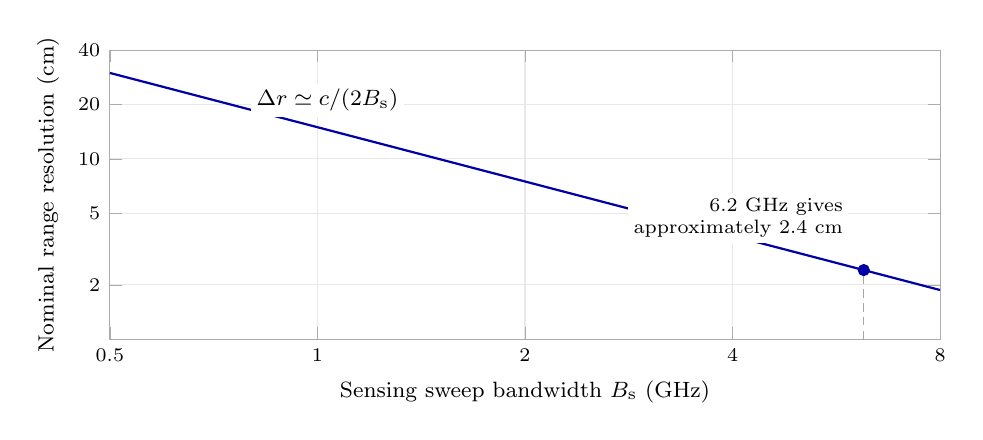
\begin{tikzpicture}
\begin{axis}[
  width=\columnwidth,height=5.25cm,
  xmin=0.5,xmax=8,ymin=1,ymax=40,
  xmode=log,ymode=log,
  xlabel={Sensing sweep bandwidth $B_{\mathrm{s}}$ (GHz)},
  ylabel={Nominal range resolution (cm)},
  xtick={0.5,1,2,4,8},xticklabels={0.5,1,2,4,8},
  ytick={2,5,10,20,40},yticklabels={2,5,10,20,40},
  tick label style={font=\scriptsize},
  label style={font=\footnotesize},
  grid=major,grid style={gray!18},
  axis line style={gray!65},tick style={gray!65},
  minor tick num=0,clip=false]
\addplot[blue!65!black,thick,domain=0.5:8,samples=100] {14.9896229/x};
\addplot[only marks,mark=*,mark size=2pt,blue!65!black]
  coordinates {(6.2,2.417681113)};
\draw[densely dashed,gray!70] (axis cs:6.2,1) -- (axis cs:6.2,2.417681113);
\node[anchor=south west,font=\footnotesize,fill=white,inner sep=2pt]
  at (axis cs:0.8,17) {$\Delta r \simeq c/(2B_{\mathrm{s}})$};
\node[anchor=south east,font=\scriptsize,align=right,fill=white,inner sep=2pt]
  at (axis cs:5.9,3.4) {6.2 GHz gives\\approximately 2.4 cm};
\end{axis}
\end{tikzpicture}

\caption{Calculated nominal range resolution for an ideal two-way,
bandwidth-limited measurement in air. The curve uses
$\Delta r=c/(2B_{\mathrm{s}})$. The marked 6.2~GHz sweep corresponds to
approximately 2.4~cm, as reported for the waveform in
\cite{OISAC_SCR00083}. The calculation describes the nominal separation scale
for two targets.}
\label{fig:bandwidth_resolution}
\end{figure}

Estimation error answers how closely an estimated parameter matches its
reference value. For $N$ range estimates, the root mean square error (RMSE) is
\begin{equation}
\mathrm{RMSE}_{r}=
\sqrt{\frac{1}{N}\sum_{i=1}^{N}(\hat r_i-r_i)^2}.
\label{eq:ranging_rmse}
\end{equation}
Here, $\hat r_i$ is the estimated range and $r_i$ is its reference value for
observation $i$, with both expressed in the same units.
A maximum absolute error describes a different statistic. The same
6.2~GHz experiment reports a maximum ranging error of 0.55~cm for static
targets at 20--45~cm \cite{OISAC_SCR00083}. This smaller error is consistent
with estimating one target more precisely than the nominal separation scale
for two targets. Practical resolution is established through a two-target
measurement. A theoretical estimation bound instead describes the limit
implied by its observation and noise model, which must be specified when
comparing it with measured error \cite{Wen2024OISACArchitectures}.

The sensing task also determines the meaning of a spatial dimension.
Fiber spatial resolution describes localization along the cable, while gauge
length specifies the separation over which differential phase is evaluated.
The fiber example in Table~\ref{tab:section2_quantitative_examples} reports
both quantities for this reason \cite{OISAC_SCR00057}.
Visible-light localization likewise separates lateral and depth performance.
Its ability to distinguish displacements along either direction is separate
from the rate at which a moving receiver's location is updated
\cite{OISAC_SCR00196}.

Signal quality must likewise be tied to a point in the receiver chain.
The optical signal-to-noise ratio (OSNR) compares optical signal and
noise power in a stated reference bandwidth before photodetection. Electrical
signal-to-noise ratio (SNR) depends on the detector, noise model, and electrical processing bandwidth.
Launch power and received power similarly refer to different locations in
Fig.~\ref{fig:joint_evidence_anatomy}. These distinctions explain why equal
numbers in decibels need not represent equal receiver conditions
\cite{OISAC_SCR00220,OISAC_SCR01180}.
Once these meanings and measurement points are fixed, communication and
sensing outcomes can be related to the setting that produced them.

\subsection{Joint Operating Points and Performance Interpretation}
\label{sec:joint_performance_interpretation}

A joint operating point links a shared design setting to both communication
and sensing outcomes under a common, identified condition set. The results
may come from one acquisition or from tests that explicitly retain the
conditions needed for the claimed relationship. A claim of simultaneous
operation additionally requires evidence that both functions operate together.
Shared hardware alone establishes where integration occurs, while the
performance relation depends on this connection between outcomes and settings.

Table~\ref{tab:section2_quantitative_examples} illustrates the meanings of
reported measures and their evaluation conditions in three systems.
Its rows collect results from the respective studies, including separate
tests, and should be read as metric examples rather than single jointly
measured operating points. The distinction preserves the contribution of
each experiment while identifying which values can be interpreted together.

\begin{table*}[!t]
\caption{Representative O-ISAC configurations and the physical meaning of
their reported performance measures}
\label{tab:section2_quantitative_examples}
\centering
\begingroup
\footnotesize
\setlength{\tabcolsep}{4pt}
\renewcommand{\arraystretch}{1.15}
\begin{tabularx}{\textwidth}{@{}
>{\raggedright\arraybackslash}p{0.10\textwidth}
>{\raggedright\arraybackslash}p{0.25\textwidth}
>{\raggedright\arraybackslash}p{0.19\textwidth}
>{\raggedright\arraybackslash}p{0.23\textwidth}
>{\raggedright\arraybackslash}X@{}}
\toprule
\textbf{System / ref.} &
\textbf{Signal and test configuration} &
\textbf{Communication measure} &
\textbf{Sensing measure and setting} &
\textbf{Technical distinction} \\
\midrule
Fiber\newline\cite{OISAC_SCR00057} &
40~km fiber. Two 30~GBaud 16-QAM subcarriers and a 500~MHz LFM probe.
A 200~Hz vibration is applied to a 1~m fiber segment. &
Reported $2\times120$~Gbit/s during concurrent sensing.
The probe-power sweep holds communication launch power at 0~dBm. &
Reported 1~m nominal spatial resolution.
Differential phase uses a 10~m gauge length.
Probe pre-compensation improves vibration-spectrum SNR by 2.4~dB. &
Span, spatial resolution, and gauge length have different roles.
The 2.4~dB gain belongs to the pre-compensation comparison. \\
\addlinespace[4pt]
Visible light\newline\cite{OISAC_SCR00196} &
225~mW white laser diode and a 1~GHz receiver.
Structured illumination covers $0.6\times0.6$~m at 2~m distance. &
Estimated data rate averages 3.35~Gbit/s across patterns,
with a 3.16--3.52~Gbit/s range. &
Separate tests resolve 1~mm lateral and approximately 4~cm depth
displacements. Dynamic localization operates at 39~frames/s. &
The pattern-averaged rate and the static and dynamic localization values
come from distinct tests. \\
\addlinespace[4pt]
Photonic THz\newline\cite{OISAC_SCR00083} &
262.1--268.3~GHz joint ASK/FMCW signal.
The 6.2~GHz sweep lasts 400~ns per chirp.
Communication is evaluated over 1~m. &
15~Gbit/s ASK with measured BER $2.97\times10^{-3}$.
The source reports approximately 36.2~GHz total occupied bandwidth. &
Nominal range resolution is approximately 2.4~cm.
Maximum ranging error is 0.55~cm for static targets at 20--45~cm,
using a separate receiver configuration. &
Sweep bandwidth differs from occupied bandwidth.
Ranging error differs from resolution, and target distance differs
from communication distance. \\
\bottomrule
\end{tabularx}
\par\vspace{3pt}
\noindent\parbox{\textwidth}{\raggedright\footnotesize
Values retain their source definitions and evaluation settings. Nominal
resolution is distinguished from measured error. Values within a row can
come from separate tests and do not by themselves define a joint operating
point. Rates estimated from signal quality are distinct from delivered
throughput.\par
QAM denotes quadrature amplitude modulation and LFM denotes linear frequency
modulation.\par
ASK denotes amplitude-shift keying and FMCW denotes frequency-modulated
continuous wave. BER denotes bit error rate and SNR denotes signal-to-noise
ratio.\par}
\endgroup
\end{table*}

The clearest performance link is a controlled change in a shared factor.
In the fiber example, increasing sensing-probe power at fixed communication
launch power raises sensing SNR while increasing the BER of both data
subcarriers \cite{OISAC_SCR00057}. This is a within-study power tradeoff.
The total launch power is not held fixed in this sweep.
The pre-compensation gain listed in the table comes from a separate comparison
using the communication receiver's response estimate.
The two comparisons reveal resource competition and a benefit of cooperation
under their respective conditions.

The other examples show why simultaneous signal generation and paired
performance measurements require separate interpretation. The THz waveform
carries data and a sensing sweep together, but communication and ranging
are evaluated with different receiver configurations \cite{OISAC_SCR00083}.
The visible-light study also demonstrates simultaneous data reception and
dynamic localization, while the table's rate average and spatial resolving
tests describe distinct evaluations \cite{OISAC_SCR00196}.
The common waveform supports integration in both cases, and each numerical
relationship retains its own test configuration.

Once both outcomes can be evaluated for a shared setting, joint design can
express the choice as a constrained problem. An illustrative
sensing-oriented formulation is
\begin{equation}
\begin{aligned}
\min_{\boldsymbol{u}\in\mathcal{U}}\quad&
\mathrm{RMSE}_{s}(\boldsymbol{u})\\
\text{subject to}\quad&
R_{\mathrm{net}}(\boldsymbol{u})\geq R_0,\\
&\mathrm{BER}(\boldsymbol{u})\leq\epsilon_b ,
\end{aligned}
\label{eq:joint_design_service_floor}
\end{equation}
where $\mathrm{RMSE}_{s}$ is the root mean square error in the selected
sensing quantity. The vector $\boldsymbol{u}$ contains the shared design variables, and
$\mathcal{U}$ imposes power, bandwidth, and hardware constraints.
The service requirements $R_0$ and $\epsilon_b$ fix the communication
performance that must be retained. This formulation illustrates a service
constraint, without assuming that every cited study solves this problem.
A communication-oriented formulation instead maximizes a communication
objective subject to a sensing requirement. A Pareto analysis examines
settings for which improving one selected objective requires worsening the
other within the feasible set
\cite{Wen2024OISACArchitectures,Lyu2026PhotonicTHzWaveforms}.
Establishing that frontier requires evaluating the feasible alternatives.
A collection of separately reported best values does not establish it.

Interpreting results across studies adds physical and measurement conditions
to this design view. Numerical comparisons require independent studies with
compatible tasks, metric definitions, and measurement points. Their operating
conditions and baselines must support the particular comparison, and a joint
claim requires both outcomes to be linked to the shared setting.
For an integration-gain comparison, a separate-function baseline must preserve
the relevant resource budget and task conditions. Otherwise, a change in
available power or measurement time can be mistaken for a gain due to sharing.
When magnitudes are not directly comparable, a recurring mechanism can still
explain a design choice, with each result retained in its own context.

The same condition set also determines what further evaluation can establish.
Simulation predicts behavior under a model, while laboratory and field tests
probe the system under their respective physical conditions.
Section~\ref{sec:validation_reproducibility} examines that validation evidence,
and Section~\ref{sec:discussion_roadmap} derives priorities for paired tests
under disturbances and against separate-function baselines.

The study-selection method follows in
Section~\ref{sec:review_methods}, while
Sections~\ref{sec:optical_modality_families} and~\ref{sec:tradeoffs}
use these foundations to examine architectures and joint-design results.

\FloatBarrier
